\documentclass[tikz,border=5]{standalone}
\usepackage{tikz}
\usetikzlibrary{shapes.geometric, arrows, positioning, fit, calc}

\begin{document}
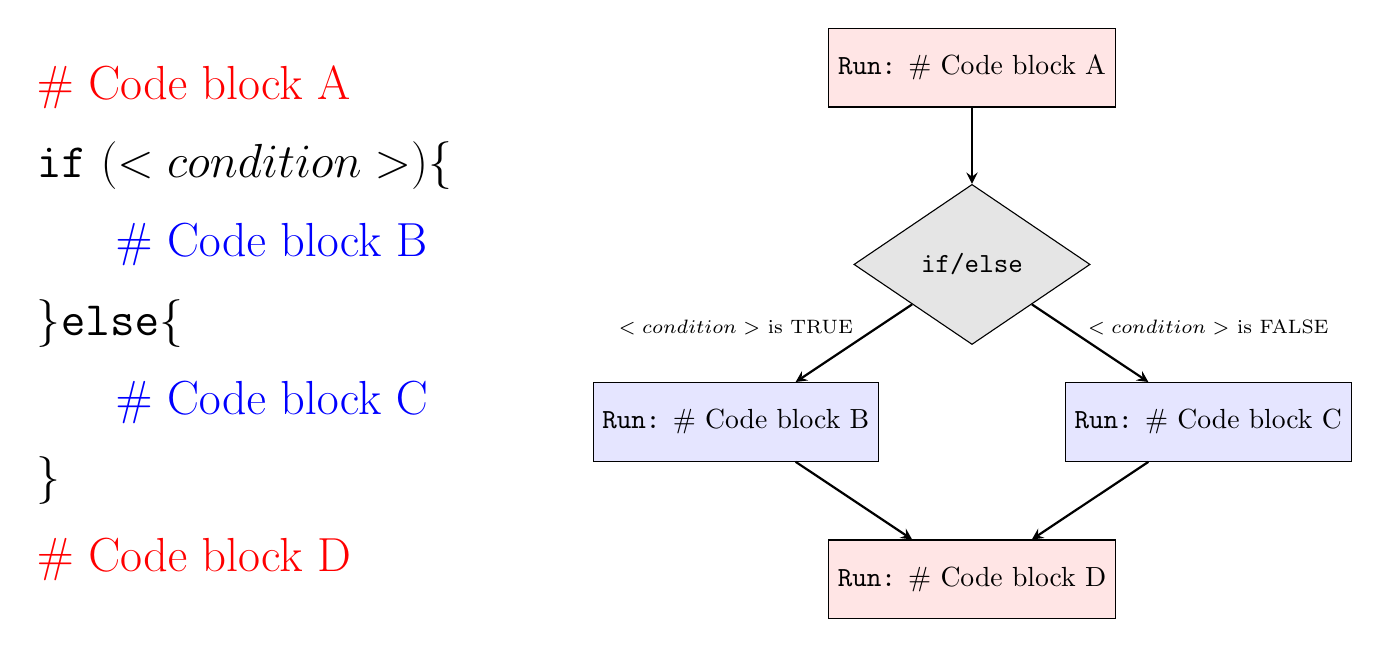
\begin{tikzpicture}
	
	\tikzstyle{process1} = [rectangle, minimum width=3cm, minimum height=1cm, text centered, draw=black, fill=red!10]
	\tikzstyle{process2} = [rectangle, minimum width=3cm, minimum height=1cm, text centered, draw=black, fill=blue!10]
	\tikzstyle{decision} = [diamond, minimum width=3cm, minimum height=1cm, text centered, draw=black, fill=black!10]
	\tikzstyle{arrow} = [thick,->,>=stealth]

	\node[anchor = west, color = red] at (0,0.25) {\LARGE\# Code block A};
	\node[anchor = west, color = black] at (0,-0.75) {\LARGE\texttt{if} $(<condition>)\{$};
	\node[anchor = west, color = blue] at (1,-1.75) {\LARGE\# Code block B};
	\node[anchor = west, color = black] at (0,-2.75) {\LARGE$\}$\texttt{else}$\{$};
	\node[anchor = west, color = blue] at (1,-3.75) {\LARGE\# Code block C};
	\node[anchor = west, color = black] at (0,-4.75) {\LARGE$\}$};
	\node[anchor = west, color = red] at (0,-5.75) {\LARGE\# Code block D};
	
	\node (pro1) [process1] at (12,0.5) {\texttt{Run:} \# Code block A};
	\node (desc2) [decision] at (12,-2) {\texttt{if/else}};
	\node (pro2) [process2] at (9,-4) {\texttt{Run:} \# Code block B};
	\node (pro3) [process2] at (15,-4) {\texttt{Run:} \# Code block C};
	\node (pro4) [process1] at (12,-6) {\texttt{Run:} \# Code block D};
	
	\node at (9, -2.8) {\scriptsize $<condition>$ is TRUE};
	\node at (15, -2.8) {\scriptsize $<condition>$ is FALSE};
	\draw [arrow] (pro1) -- (desc2);
	\draw [arrow] (desc2) -- (pro2);
	\draw [arrow] (desc2) -- (pro3);
	\draw [arrow] (pro3) -- (pro4);
	\draw [arrow] (pro2) -- (pro4);
	
	
\end{tikzpicture}
\end{document}